% !TEX encoding = UTF-8
% !TEX TS-program = pdflatex
% !TEX root = ../tesi.tex

%**************************************************************
\chapter{Verifica e validazione}
\label{cap:testing} 

\section{Analisi statica}
L'analisi statica è stata realizzata grazie all'utilizzo di SonarQube \cite{site:sonarqube} e veniva eseguita ad ogni occorrenza di una build di Jenkins.
I problemi che SonarQube può segnalare, possono essere di tre tipi:
\begin{itemize}
    \item \bd{bug}: un errore nel codice che richiede di essere corretto il prima possibile;
    \item \bd{vulnerabilità}: un punto nel codice che è aperto agli attacchi;
    \item \bd{codesmell}:  un problema che rende il codice confuso e difficile da manutenere.
\end{itemize}
Ognuno dei quali può avere un grado di severità differente, ordinate dalla più alla meno importante:
\begin{itemize}
    \item \bd{BLOCKER}
    \item \bd{CRITICAL}
    \item \bd{MAJOR}
    \item \bd{MINOR}
    \item \bd{INFO}.
\end{itemize}

La maggior parte dei problemi segnalati da SonarQube durante il progetto, erano codesmell con severità MINOR o MAJOR.
La figura \ref{sonarMAJORissue} ne riporta un esempio.

\clearpage

\begin{figure}[H]
    \centering
    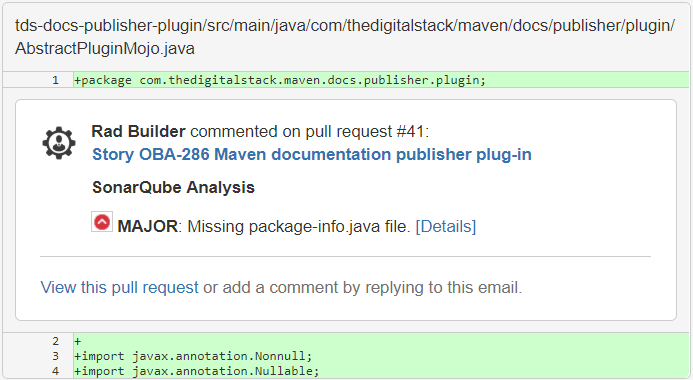
\includegraphics[width=\textwidth]{immagini/major-issue.png}\\
    \caption{Esempio di SonarQube MAJOR issue}
    \label{sonarMAJORissue}
\end{figure}

Per il termine del progetto, la totalità di quelli etichettati come MAJOR sono stati risolti, come richiesto dalle norme aziendali relative al codice, e anche molti dei MINOR.
 

\section{Test di unità}

L'attività di testing per quel che riguarda i test di unità è stata svolta utilizzando principalmente due framework: JUnit e Mockito.

    \subsection{JUnit}
    JUnit è il framework ideale per sviluppare i test di unità in Java.
    Esso fornisce notazioni \cite{site:junit-annotation} essenziali quali:
    \begin{itemize}
        \item \txt{Test} per indicare che il metodo rappresenta un test \cite{site:junit-test};
        \item \txt{Before} per creare gli oggetti comuni a più test prima della loro esecuzione;
        \item \txt{Ignore} per ignorare temporaneamente un test.
    \end{itemize}
    
    % \begin{figure}[H]
    %     \centering
    %     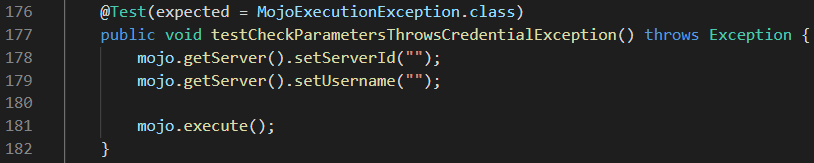
\includegraphics[width=\textwidth]{immagini/screenTest.png}\\
    %     \caption{Esempio di test}
    %     \label{screenTest}
    % \end{figure}
    Viene qui di seguito riportato un esempio:
    \begin{lstlisting} 
    @Test(expected = MojoExecutionException.class)
    public void testCheckParametersThrowsCredentialException() throws Exception {
        mojo.getServer().setServerId("");
        mojo.getServer().setUsername("");

        mojo.execute();
    }
    \end{lstlisting}
    La notazione Test viene qui usata in aggiunta al tipo di eccezione che il test si aspetta.
    Questo perché, in questo caso in particolare, il test verifica che venga tirata un'eccezione durante l'esecuzione del plugin, perché sia serverId che username sono stringhe vuote, quindi non c'è nessun modo per ottenere le credenziali corrette. \\

    Sono stati utilizzati inoltre i classici metodi di \txt{org.junit.Assert} come \txt{assertEquals()}, \txt{assertNull()}, \txt{assertTrue()} ecc, utili per determinare lo stato di un test case.

    \subsection{Mockito}
    Mockito è un mock framework molto popolare che può essere usato in congiunzione a JUnit \cite{site:mockito}. 
    Ciò vuol dire che Mockito consente la creazione e configurazione di mock object.
    I mock object sono degli oggetti simulati che riproducono il comportamento degli oggetti reali in modo controllato \cite{site:mock}.
    Un programmatore crea un oggetto mock per testare il comportamento di altri oggetti, reali, ma legati ad un oggetto inaccessibile o non implementato.
    Generalmente, all'interno del progetto, questi oggetti sono per esempio il client per il mojo o il server per il client.
    Realizzare un oggetto mock in questi casi era utile per evitare di trasformare i test di unità in test d'integrazione.

    Ad esempio:

    % oppure usare verbatim
    \begin{lstlisting} 
        @Test
        public void testCreateDoc() throws Exception {
            String categoryId = "c0000";
            String docName = "Documentation";
            File archive = File.createTempFile("file", "txt");
            DocDetails doc = new DocDetails();

            ClientResponse response = mock(ClientResponse.class);
            when(response.getStatus()).thenReturn(200);
            when(response.getEntity(DocDetails.class)).thenReturn(doc);
            when(builder.put(any(Class.class))).thenReturn(response);

            DocDetails returnedDoc = client
                .createDoc(categoryId, docName, archive);

            verify(httpClient).resource(new URI(
                serverInfo.getUrl() + "rest/docs/2.0/repository/" + 
                categoryId + "/" + docName));
            assertNotNull(returnedDoc);
            verify(builder).put(any(Class.class));
        }
    \end{lstlisting}
    Come suggerisce il nome, questo test verifica il comportamento del metodo \txt{createDoc()} di DocsPluginClient.
    Grazie a Mockito è possibile determinare il comportamento desiderato di molti oggetti, per esempio della riposta proveniente da Confluence in seguito ad una richiesta (\txt{ClientResponse}).
    È possibile infatti decidere lo stato della risposta: 200 in questo caso.
    In un altro test in cui si è scelti stato 401, il test dovrebbe verificare la ricezione di un errore o un'eccezione.

    Oltre a decidere come un mock object si dovrebbe comportare, è possibile ad esempio verificare che un preciso metodo sia stato invocato.
    In questo caso, dopo che il metodo \txt{createDoc()} è stato chiamato, viene controllato che il metodo \txt{put()} sia stato invocato (ultima riga del codice).
    Questo è di grande utilità per controllare che l'oggetto sotto test si comporti come dovrebbe, chiamando i corretti metodi degli oggetti mock.


\section{Test di validazione}
Al termine dell'implementazione del prodotto, insieme all'attività di testing, si è proceduto con la verifica di tutti i casi possibili, dal punto di vista di un qualunque sviluppatore che utilizza il plugin.
Tra i casi limite, troviamo per esempio:
\begin{itemize}
    \item pubblicazione di documentazione in una categoria in cui l'utente non ha permesso di accesso;
    \item pubblicazione di documentazione in una categoria inesistente;
    \item inserimento in configurazione del nome di un file inesistente all'interno della cartella data;
    \item omissione dell'utente di inserimento in configurazione delle credenziali.
\end{itemize}
In tutti questi tentativi, il prodotto si è comportato come atteso, dando dei messaggi di errore.
Anche in tutte le altre circostanze previste, è stata verificata la corretta esecuzione del plugin. \\

Insieme agli sviluppatori senior DevOps dell'azienda e il tutor aziendale, ci si è accertati che tutte le funzionalità attese del prodotto, descritte nella sezione \S\ref{requisitiFunzionalita}, sono state concretizzate. \\
In generale si è appurato che i requisiti, nella loro totalità, siano stati soddisfatti; non soltanto quindi i requisiti di funzionalità, ma anche i requisiti esplicitati nelle sezioni successive, quali requisiti di qualità e di vincolo, dagli obbligatori agli opzionali, come la stesura dei manuali e l'adozione di tutti gli strumenti elencati.


%**************************************************************